\subsection{Messergebnisse und Auswertung}
Die Messungen wurden mit einem digitalen Oszilloskop durchgeführt. Die Zeiten und Spannungen sind nicht kontinuierlich verteilt, sie können 
nur diskrete Werte annehmen. Die Auflösung der Zeit beträgt $\Delta t = 0.02$\,\textmu s, die der Spannung $\Delta U = 0.1$\,mV. \\
TODO Gleichverteilung. %TODO Gleichverteilung
\begin{equation}
  s_t = \frac{\Delta t}{\sqrt{12}}, \qquad s_U = \frac{\Delta U}{\sqrt{12}}
\end{equation}
Beim Ablesen der Treibspannung $U_T$ wurde eine deutliche Veränderung der gemessenen Treibspannung bei unterschiedlich eingestellten 
Anzeigeoffsets beobachtet. Aus diesem Grund wurde der Fehler der Treibspannung auf $s_{U_T} = 0.4$\,V geschätzt. \\
Der Fehler auf den Abstand $d$ zwischen Lichtleiter und Messspitze wurde auf $s_d = 0.05$\,mm gesetzt.
\subsubsection{Bestimmung des Offsets \texorpdfstring{$x_0$}{x0}}
Der Abstand zwischen Messspitze und Lichtleiter wurde aufgrund des Versuchsaufbaus mit einem Offset $x_0$ gemessen. Der Offset wurde separat 
von jedem Versuchspartner einmal bestimmt. Aus den Messwerten wurde der Mittelwert bestimmt (Fehler der Einzelmessung 
$s_{x_i} = 0.2$\,mm \footnote{Die Schieblehre konnte nicht direkt angelegt werden, um den Versuchsaufbau nicht zu beschädigen. 
Dadurch ist konnte man den Offset nicht so genau bestimmen.}):
\begin{equation}
  x_0 = (1.25 \pm 0.14)\,\text{mm}
\end{equation}
\subsubsection{Variation der Nadelposition \texorpdfstring{$d$}{d}}

\begin{figure}[H]
\begin{center}
  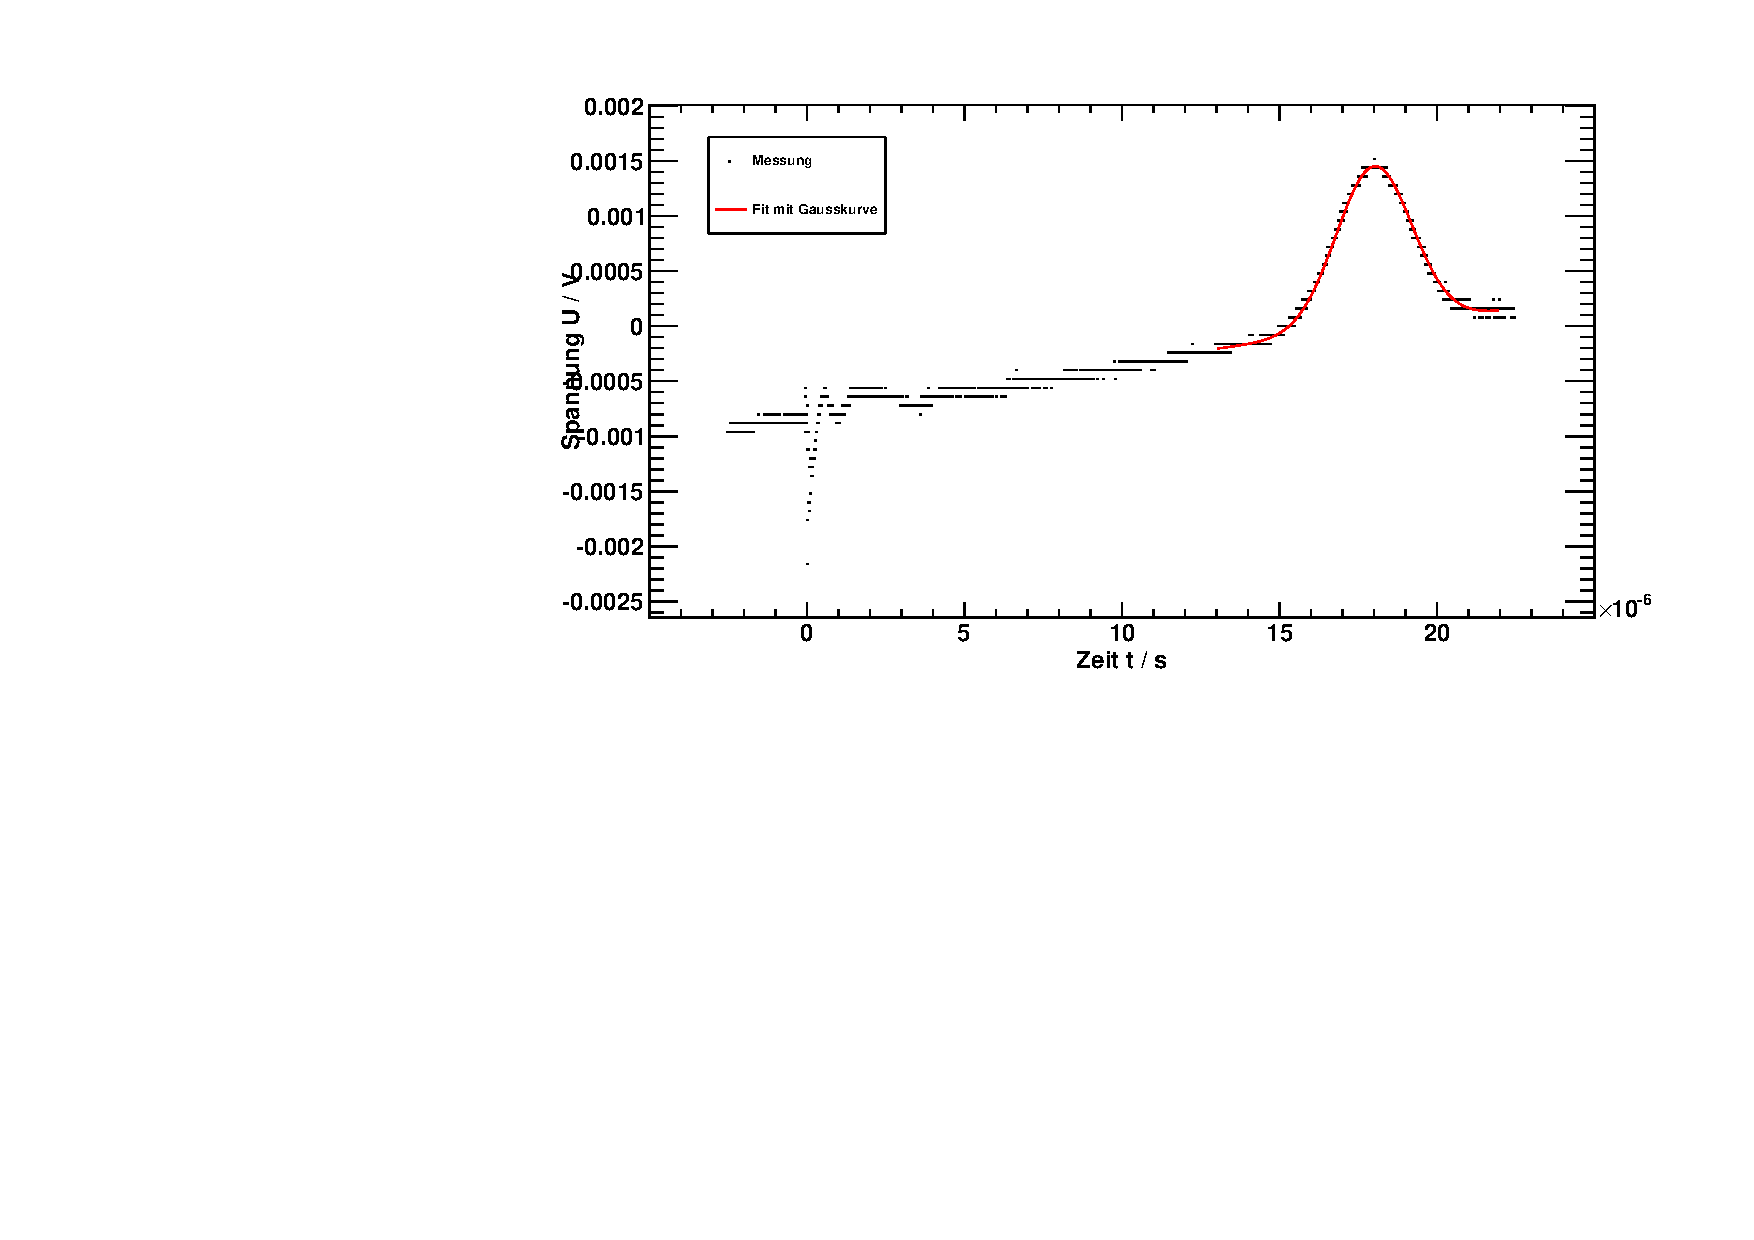
\includegraphics[width=\textwidth]{../img/part2/dist02.pdf}
  \caption{Gaußfit mit linearem Untergrund des Peaks bei $d=8.03$\,mm.}
  \label{img:d:exfit}
\end{center}
\end{figure}
\autoref{img:d:exfit} zeigt einen beispielhaften Fit in dieser Messreihe. Insgesamt wurden so 11 Messungen gefittet. Die Gleichung ergibt sich 
aus \autoref{eq:gauss} und einem linearen Untergrund:
\begin{equation}
  U(t) = a + b \cdot t + A \cdot \frac{1}{\sqrt{2  \pi  \cdot \sigma^2}} \cdot
  e^{-\frac{1}{2} \left( \frac{t - t_{\text{c}}}{\sigma^2} \right)^2}
\end{equation}
Für die weiteren Berechnungen sind für die Amplitude $A$, den zeitlichen Schwerpunkt $t_c$ und die Standardabweichung $\sigma$ die Fehler aus 
den Fits verwendet worden.
Die untergrundbereinigten Messungen (ohne Fits) sind in \autoref{img:distances} dargestellt.
\begin{figure}[H]
\begin{center}
  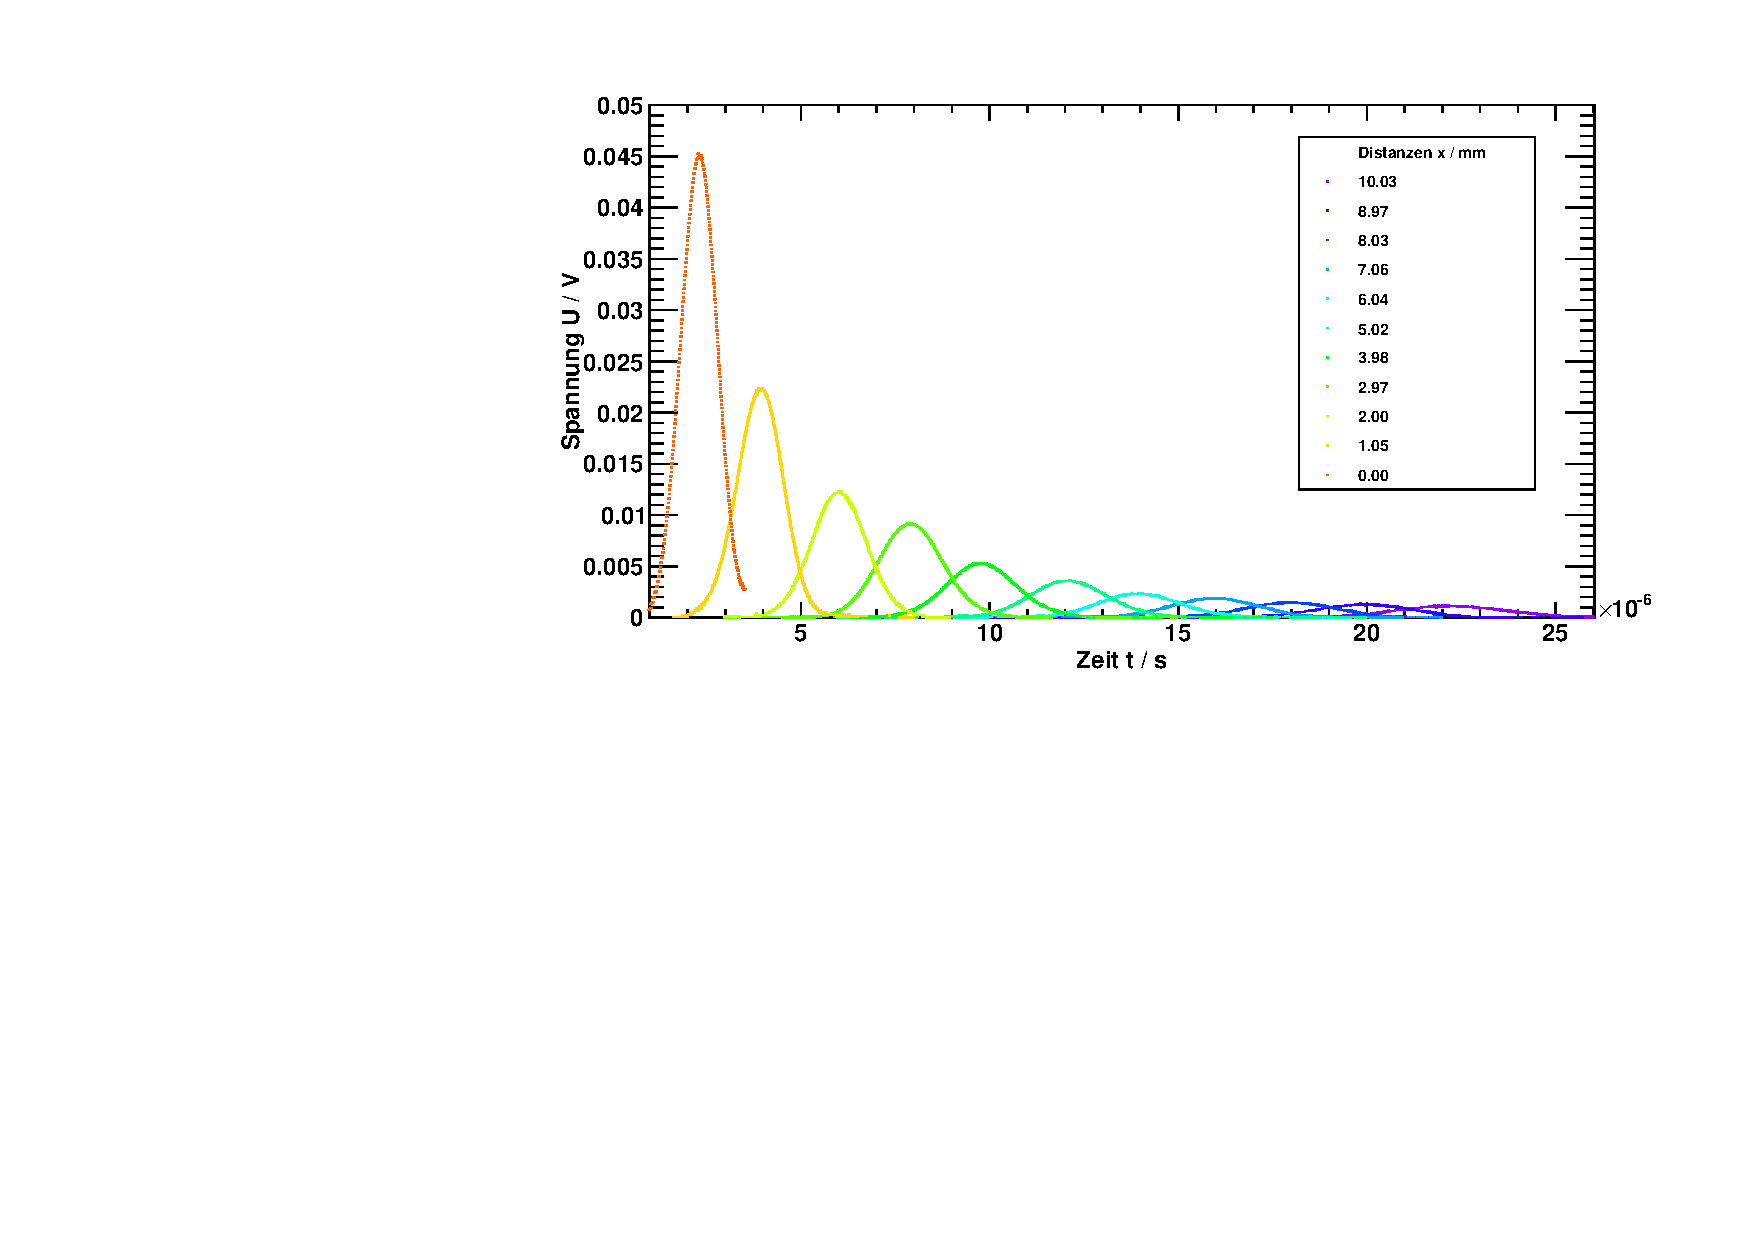
\includegraphics[width=\textwidth]{../img/part2/distances.pdf}
  \caption{Zeitlicher Verlauf der Spannungen für verschiedene Abstände $d$ zwischen Messspitze und Lichtleiter.}
  \label{img:distances}
\end{center}
\end{figure}

\paragraph{Bestimmung der Ladungsträgermobilität $\mu$}
Für jeden Gaußfit wird die Entfernung $d$ zwischen Lichtleiter und Nadelspitze über dem Zeitpunkt des Maximumdurchlaufs $t_{\text{c}}$ 
aufgetragen (\autoref{img:dist:fitxc}), da der örtliche Schwerpunkt $x_c(t)$ zum Zeitpunkt $t_c$ genau $d$ entspricht. Mit 
\autoref{eq:gaus:params} erhält man so eine proportionale Abhängigkeit des Abstandes $d$ von dem zeitlichen Schwerpunkt $t_c$ mit 
$\mu \cdot E$ als Proportionalitätskonstante.
\begin{equation}
  d = x_c(t_c) = \mu \cdot E \cdot t_c
\end{equation} 
Der so erhaltene Graph wird mit einer Geraden gefittet.
\begin{equation}
  x_c(t_c) = x_0 + m \cdot t_c
\end{equation}

\begin{figure}[H]
\begin{center}
  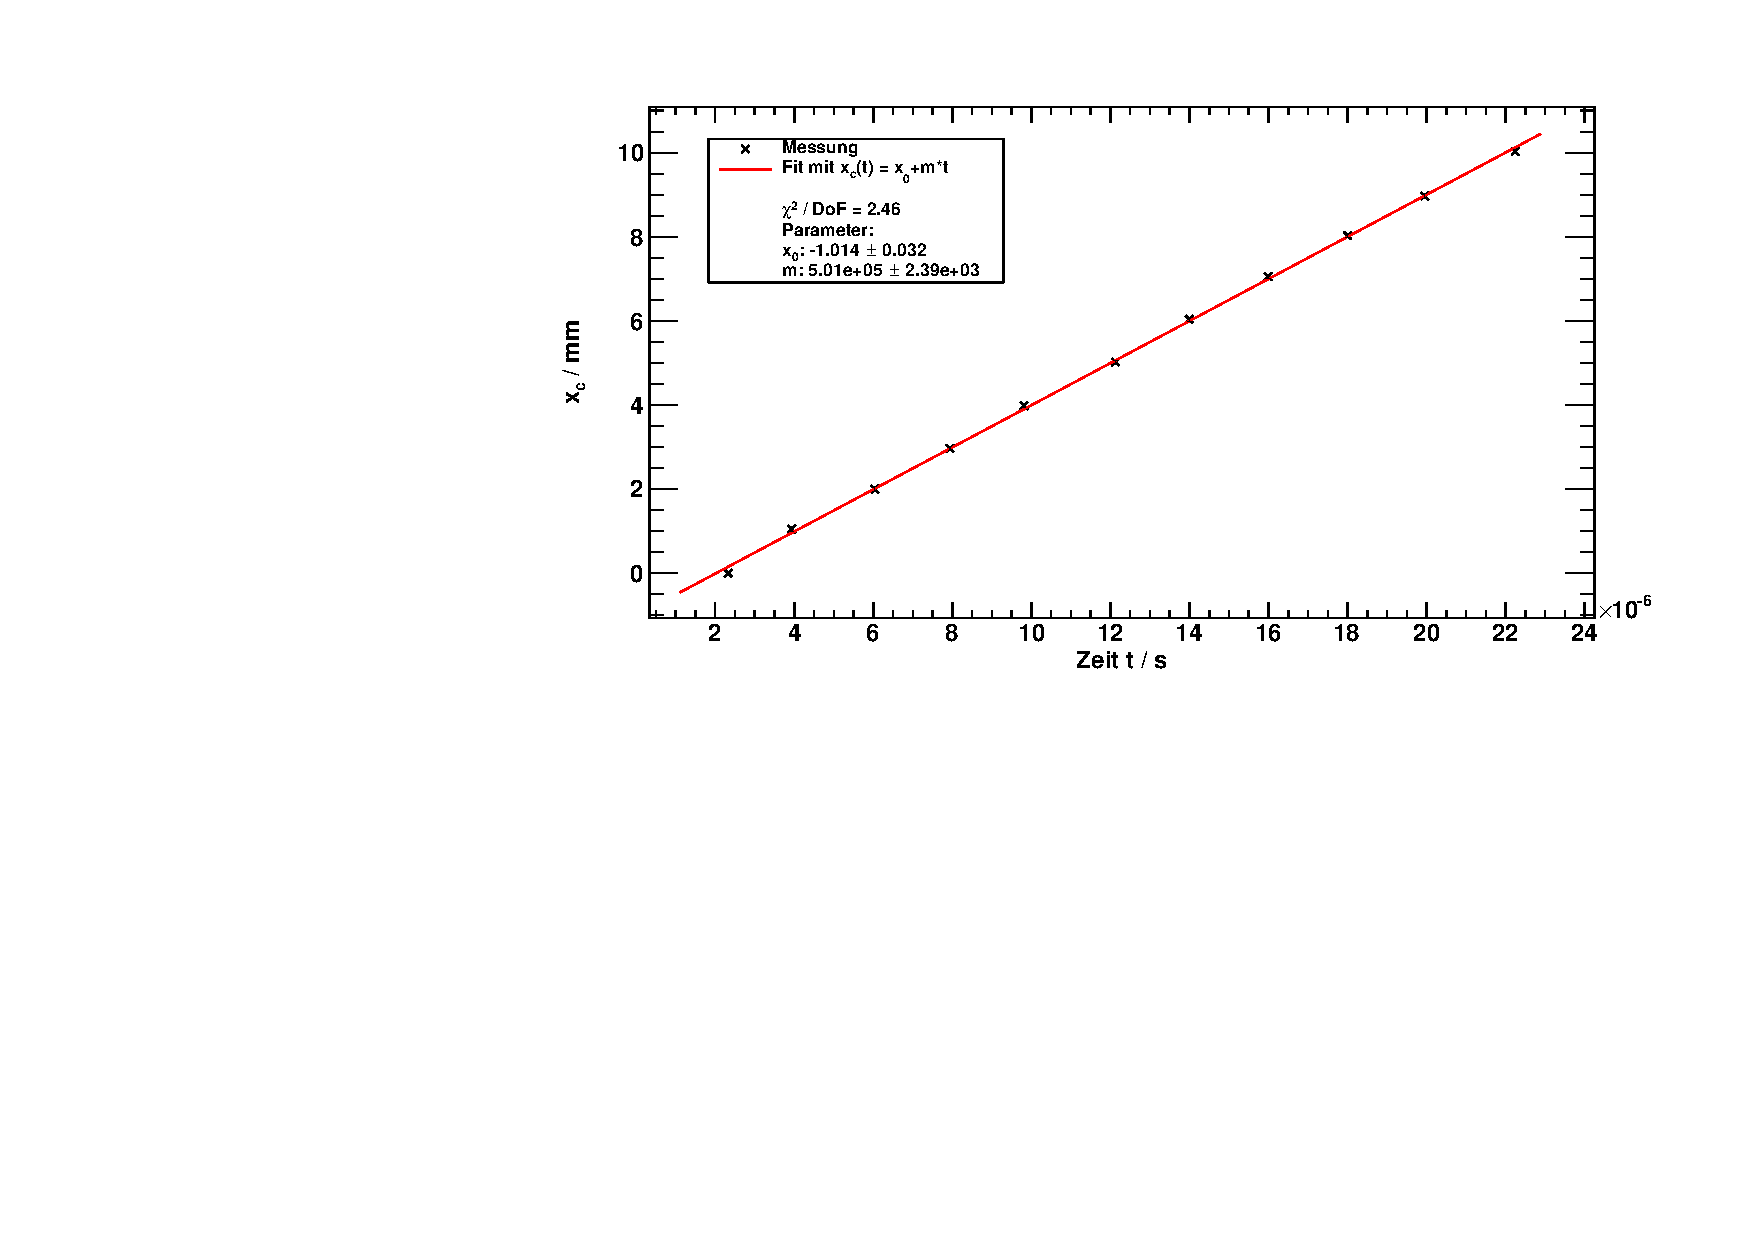
\includegraphics[width=\textwidth]{../img/part2/dist_fitXc.pdf}
  \caption{Ausgleichsgerade} %TODO caption
  \label{img:dist:fitxc}
\end{center}
\end{figure}

Der Betrag des Achsenabschnitts $|x_0| = (1.01 \pm 0.03)$\,mm stimmt innerhalb von zwei Standardabweichungen mit dem oben bestimmten Wert des 
Offsets überein.\\
Die Steigung $m$ ist das Produkt aus Ladungsträgermobilität und angelegtem E-Feld:
\begin{equation}
  \label{eq:efield}
  m = \mu \cdot E = \mu \cdot \frac{U}{d}
\end{equation}
mit $U = (48.8 \pm 0.4)$\,V und $d=30$\,mm. Man erhält mit Gauß'scher Fehlerfortpflanzung für $\mu$:
\begin{equation}
  \mu = (3079 \pm 29)\,\frac{\text{cm}^2}{\text{V} \cdot \text{s}}
\end{equation}
Dieser Wert ist gegenüber dem Literaturwert
\begin{equation}
  \mu^{\text{Lit}} = 3900\,\frac{\text{cm}^2}{\text{V} \cdot \text{s}}
\end{equation}
stark erniedrigt. Dies kann mit Gitterfehlern an der Probenoberfläche erklärt werden, da diese die Ladungsträgermobilität verringern.

\paragraph{Bestimmung der Diffusionskonstanten $D_\text{n}$}
Die aus den Fits erhaltenen Standardabweichungen $\tilde{\sigma}$ werden gemäß \autoref{eq:gauss} mit $\mu \cdot E$ multipliziert und 
in \autoref{img:dist:fitsigma} über $t_c$ aufgetragen. Die Beweglichkeit $\mu$ erhält man von oben und das E-Feld wird analog zu \autoref{eq:efield} berechnet.
Der Fit erfolgt mit \autoref{eq:gaus:params} und einem Zeitoffset $t_0$.
\begin{equation}
  \sigma(t) = \sqrt{2 \cdot D_\text{n} \cdot (t-t_0)}
\end{equation}
Der Offset könnte von einer ungenauen Triggerung auf den Laserpuls oder seine Ausdehnung verursacht werden. \\
Bei dem Fit wurde der letzte Messwert ($t=22$\,\textmu s) nicht berücksichtigt, da er offensichtlich weit neben dem Modell liegt.

\begin{figure}[H]
\begin{center}
  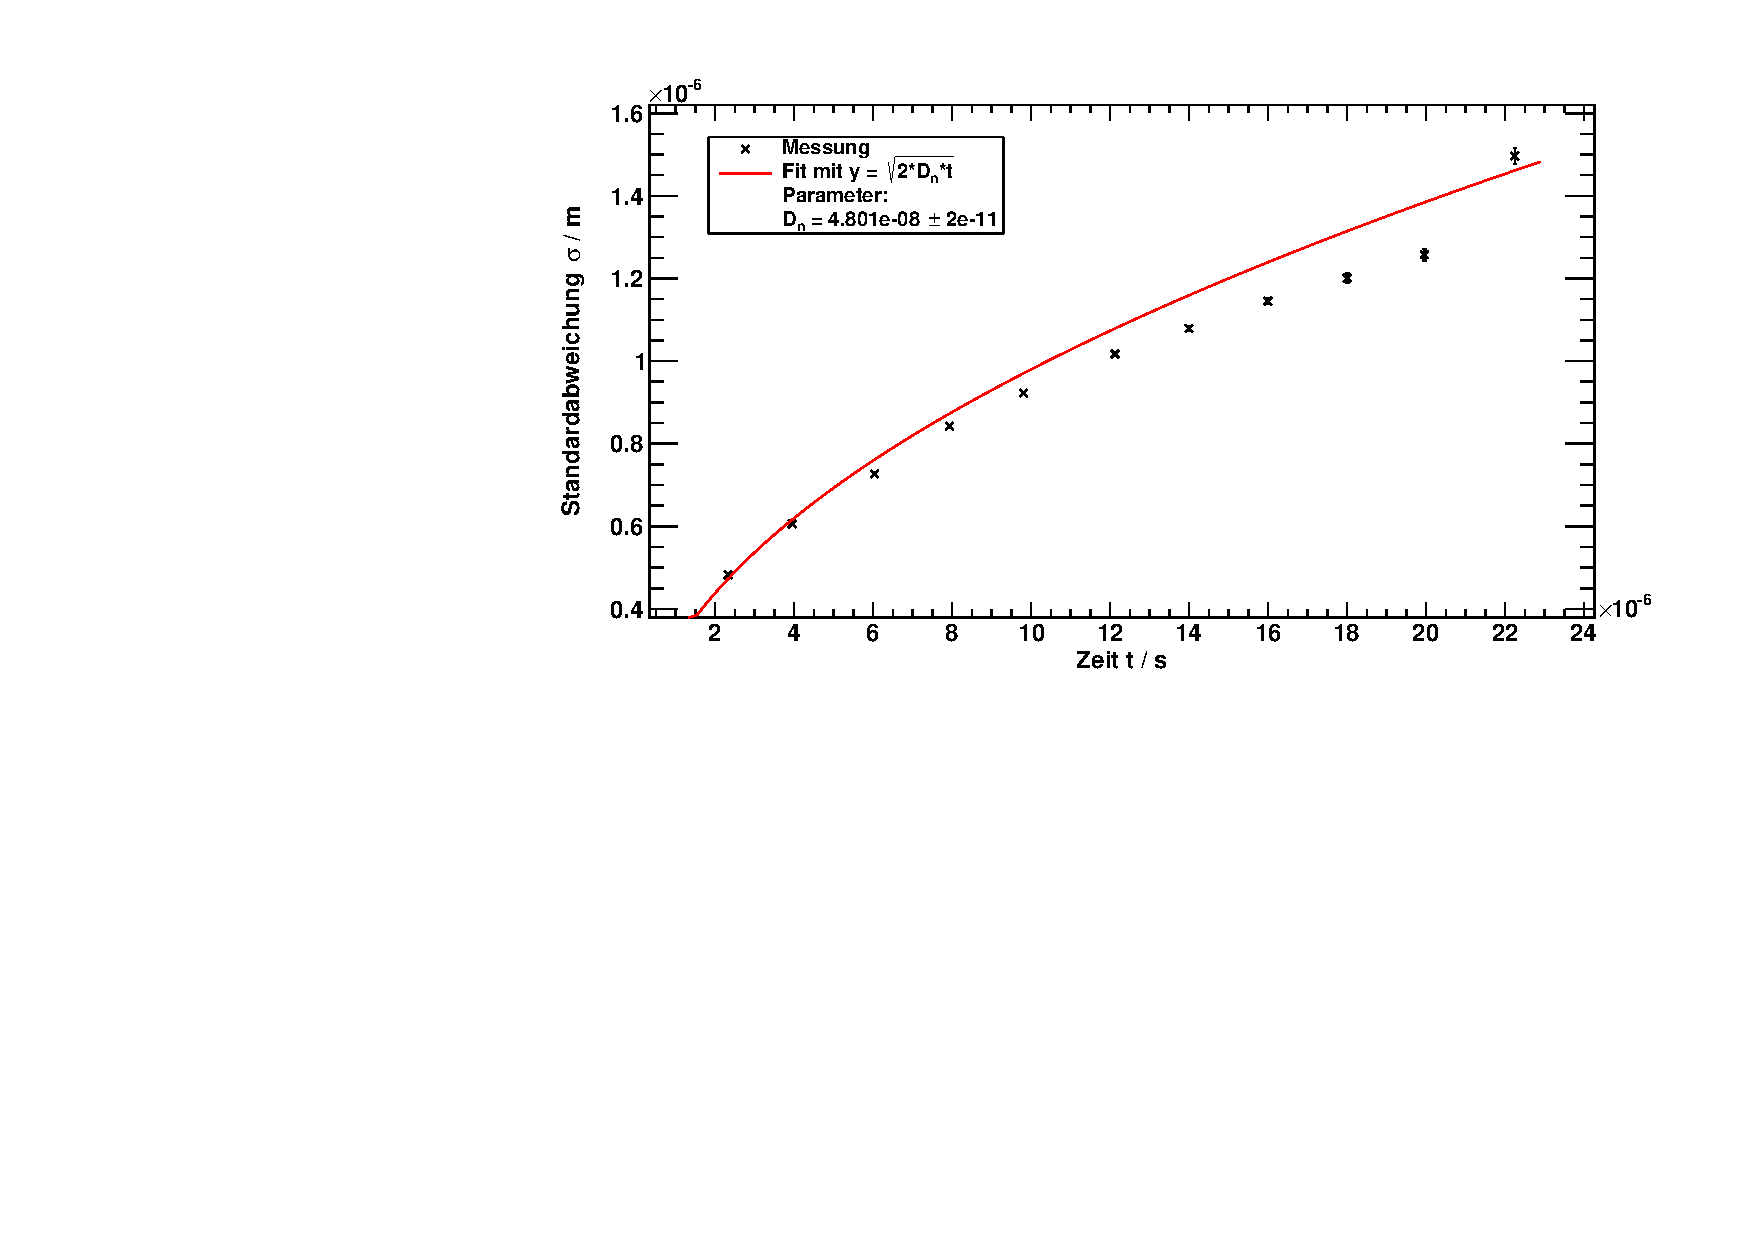
\includegraphics[width=\textwidth]{../img/part2/dist_fitSigma.pdf}
  \caption{caption}
  \label{img:dist:fitsigma}
\end{center}
\end{figure}
Man erhält für die Diffusionskonstante:
\begin{equation}
  D_\text{n} = (99.6 \pm 1.1)\,\frac{\text{cm}^2}{\text{s}}
\end{equation}
Sie stimmt innerhalb von zwei Standardabweichungen mit dem Literaturwert überein. 
\begin{equation}
  D_\text{n}^{\text{Lit}} = 101\,\frac{\text{cm}^2}{\text{s}} 
\end{equation}

\paragraph{Bestimmung der mittleren Lebensdauer $\tau_\text{n}$}
Für die Bestimmung der mittleren Lebensdauer wird der Zusammenhang aus \autoref{eq:gaus:params} mit einen konstanten Offset verwendet:
\begin{equation}
  A(t) = C \cdot e^{- \frac{t}{\tau_\text{n}}} + a
\end{equation}
Der Offset gibt einen systematischen Fehler an, der durch einen Teil des Untergrundes, welcher nicht mit der linearen Funktion oben 
berücksichtigt wurde, verursacht werden könnte. \\
Der Fehler auf die Amplituden kommt aus den Fits der einzelnen Gauß-Peaks. Jedoch muss noch berücksichtigt werden, dass jeder Peak von einem 
eigenen Laserpuls erzeugt wurde. Der relative Fehler auf die Intensität des Lasers wurde auf $s_\text{Laser, rel} = 5\%$ geschätzt. Dadurch 
lässt sich nun der Fehler auf die Amplituden mit 
\begin{equation}
  s_A = \sqrt{s_\text{Fit}^2 + s_\text{Laser, rel}^2}
\end{equation}
\begin{figure}[H]
\begin{center}
  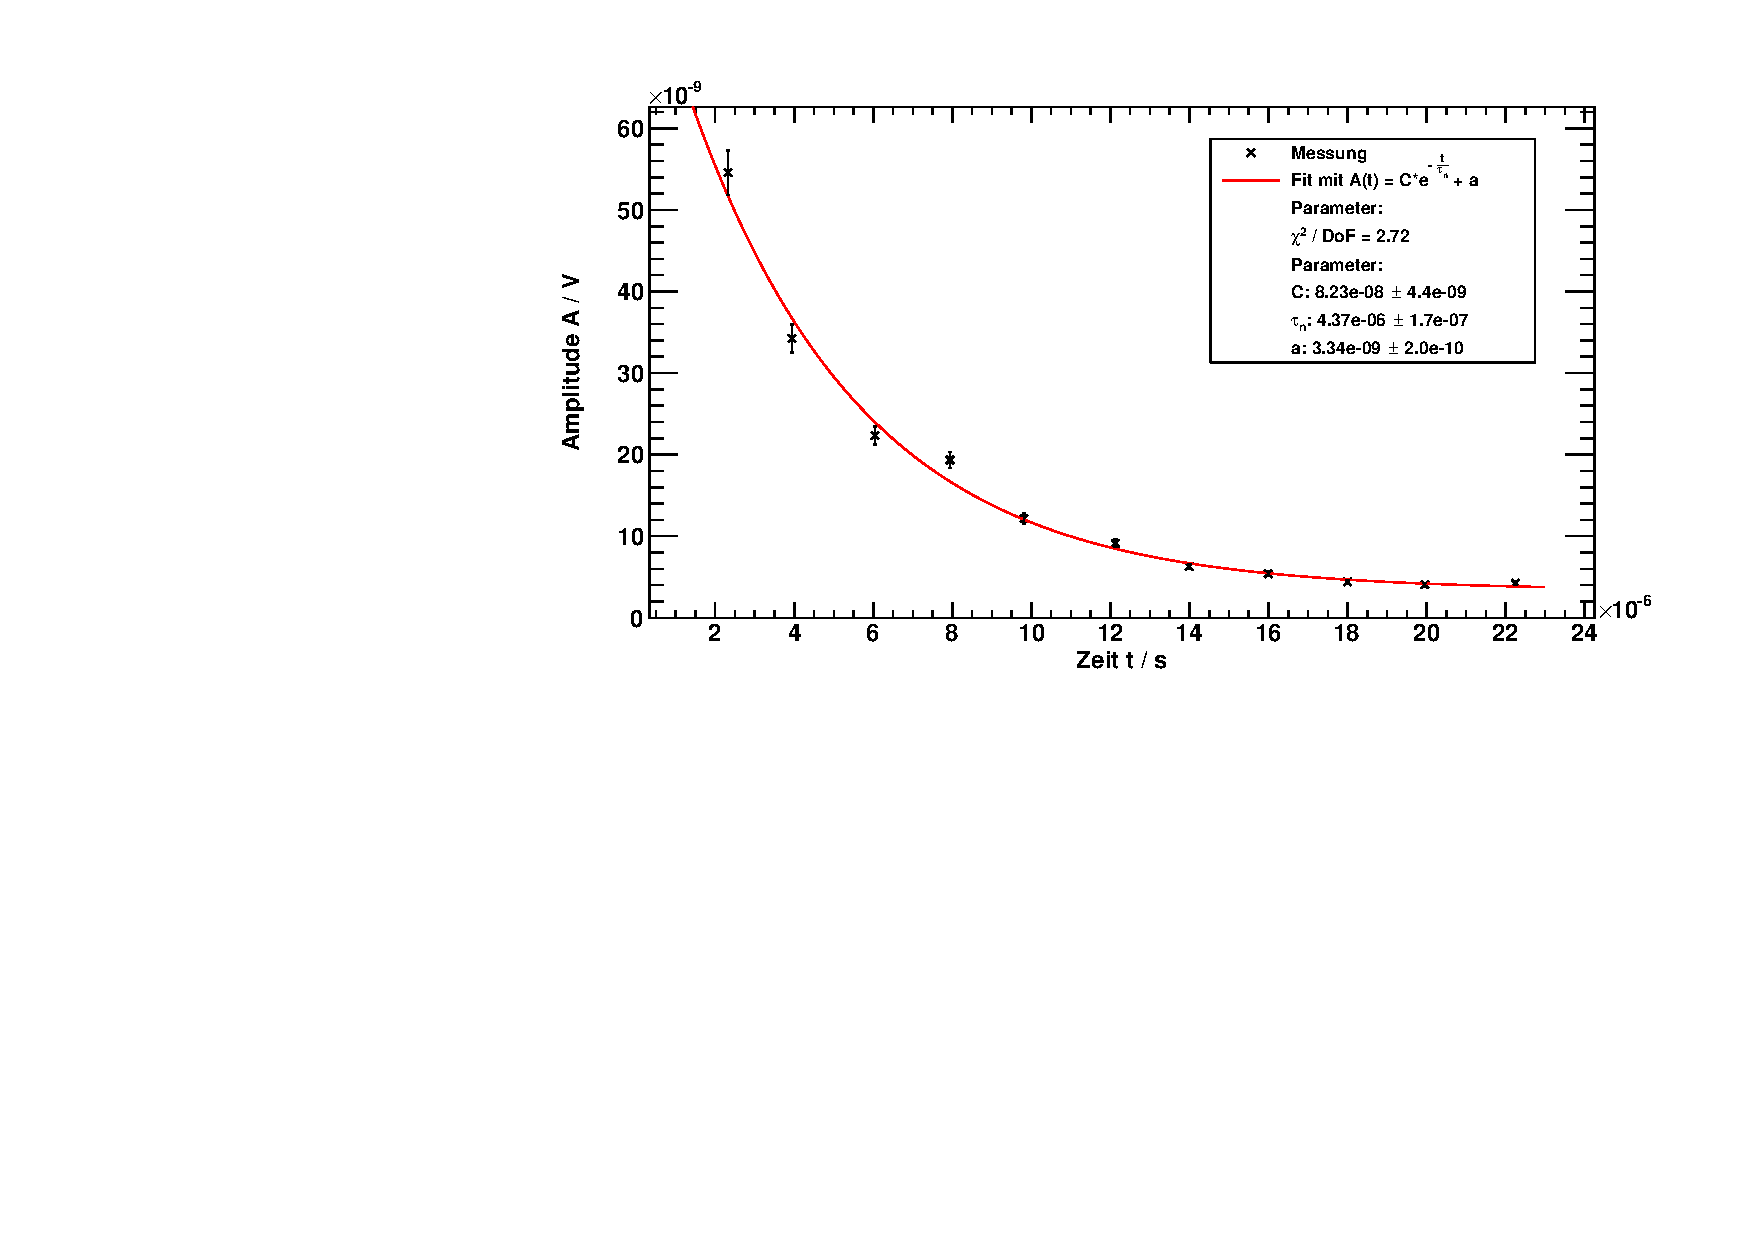
\includegraphics[width=\textwidth]{../img/part2/dist_fitA.pdf}
  \caption{caption}
  \label{img:dist:fita}
\end{center}
\end{figure}
Der Fit liefert für die mittlere Lebensdauer:
\begin{equation}
  \tau_\text{n} = (4.37 \pm 0.17)\,\text{\textmu s}
\end{equation}
Dieser Wert liegt weit unter dem Literaturwert. Die Ursache dafür ist Rekombination der Ladungsträger an oberflächlichen Gitterfehlern.
\begin{equation}
  \tau_\text{n}^\text{Lit} = (45 \pm 2)\,\text{\textmu s}
\end{equation}


\subsubsection{Variation der Treibspannung \texorpdfstring{$U_T$}{U\_T}}

\begin{figure}[H]
\begin{center}
  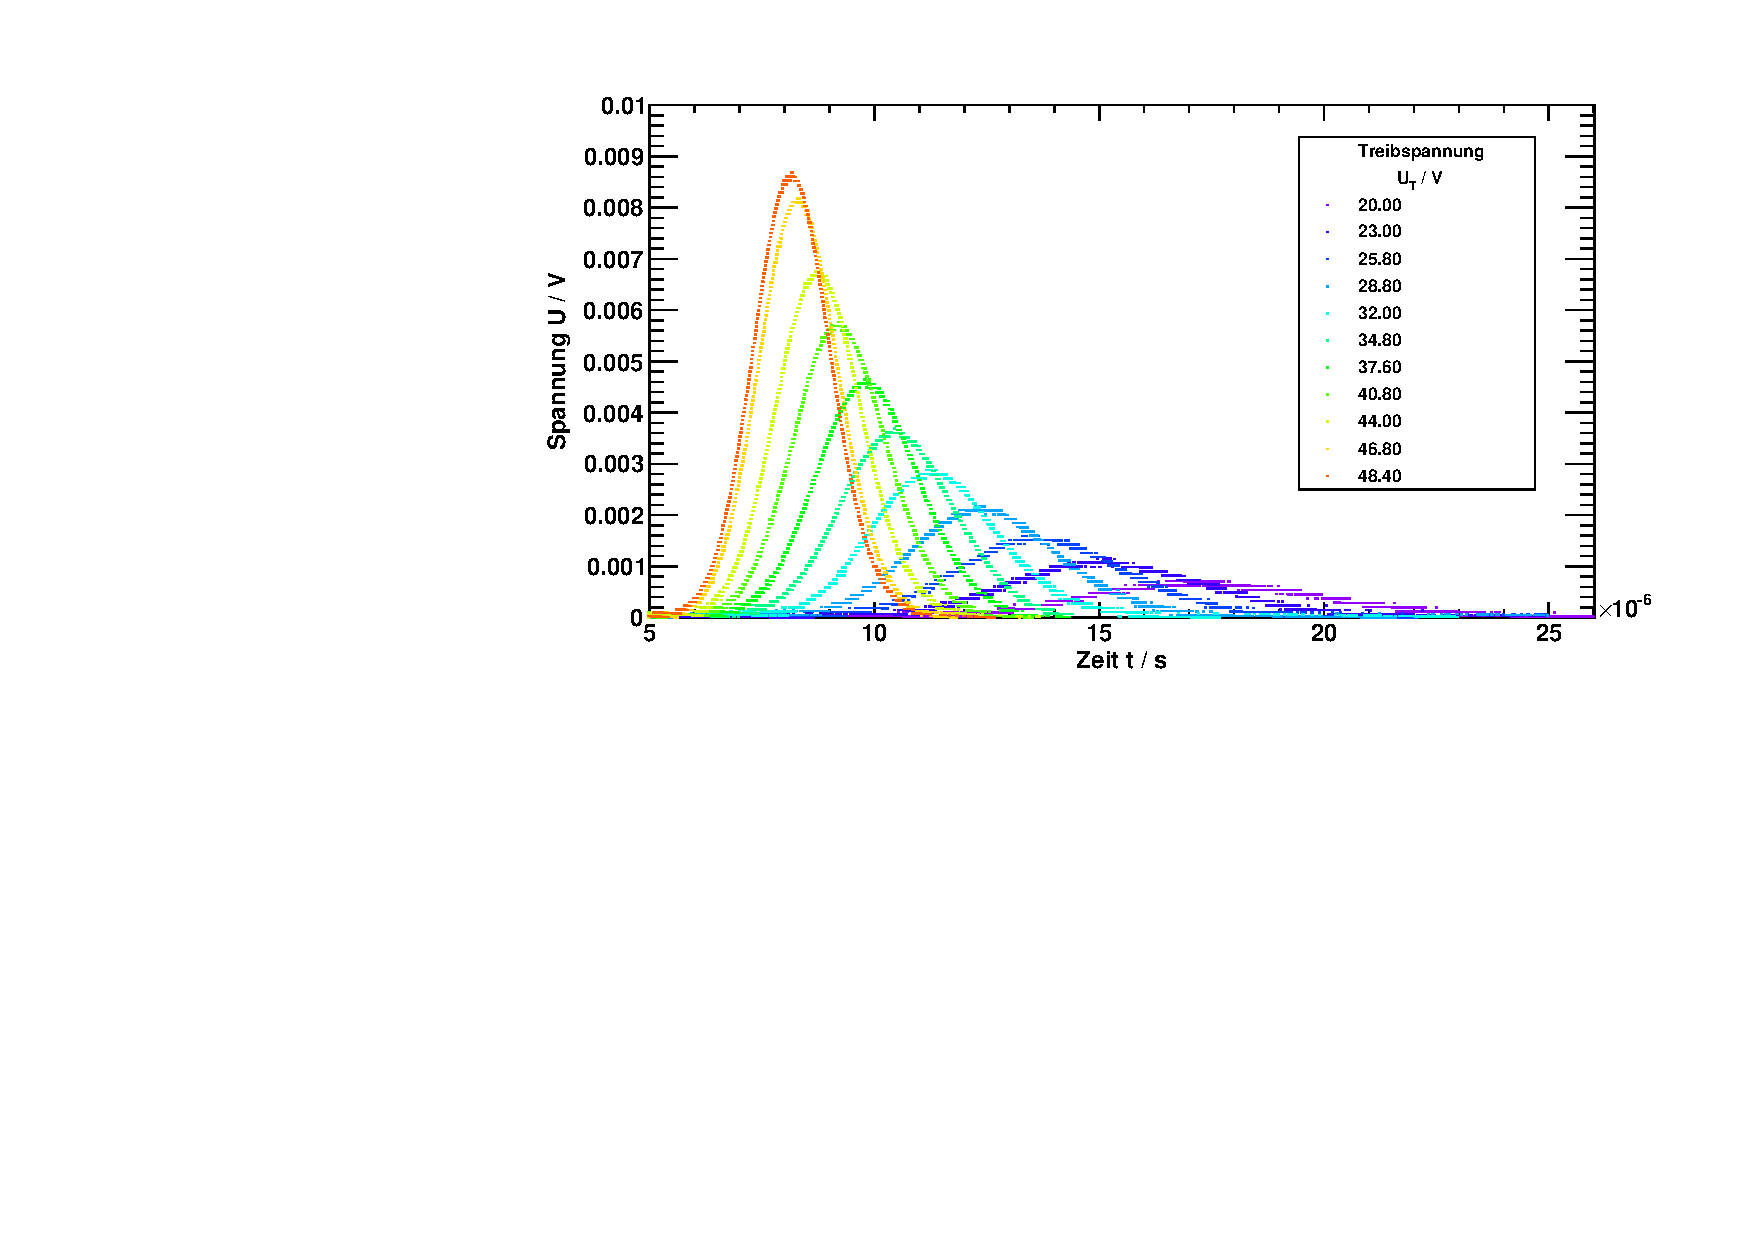
\includegraphics[width=\textwidth]{../img/part2/voltages.pdf}
  \caption{Zeitlicher Verlauf der Spannungen für verschiedene Treibspannungen $U_T$.}
  \label{img:volts}
\end{center}
\end{figure}

\paragraph{Bestimmung der Ladungsträgermobilität $\mu$} 
Platzhalter

\begin{figure}[H]
\begin{center}
  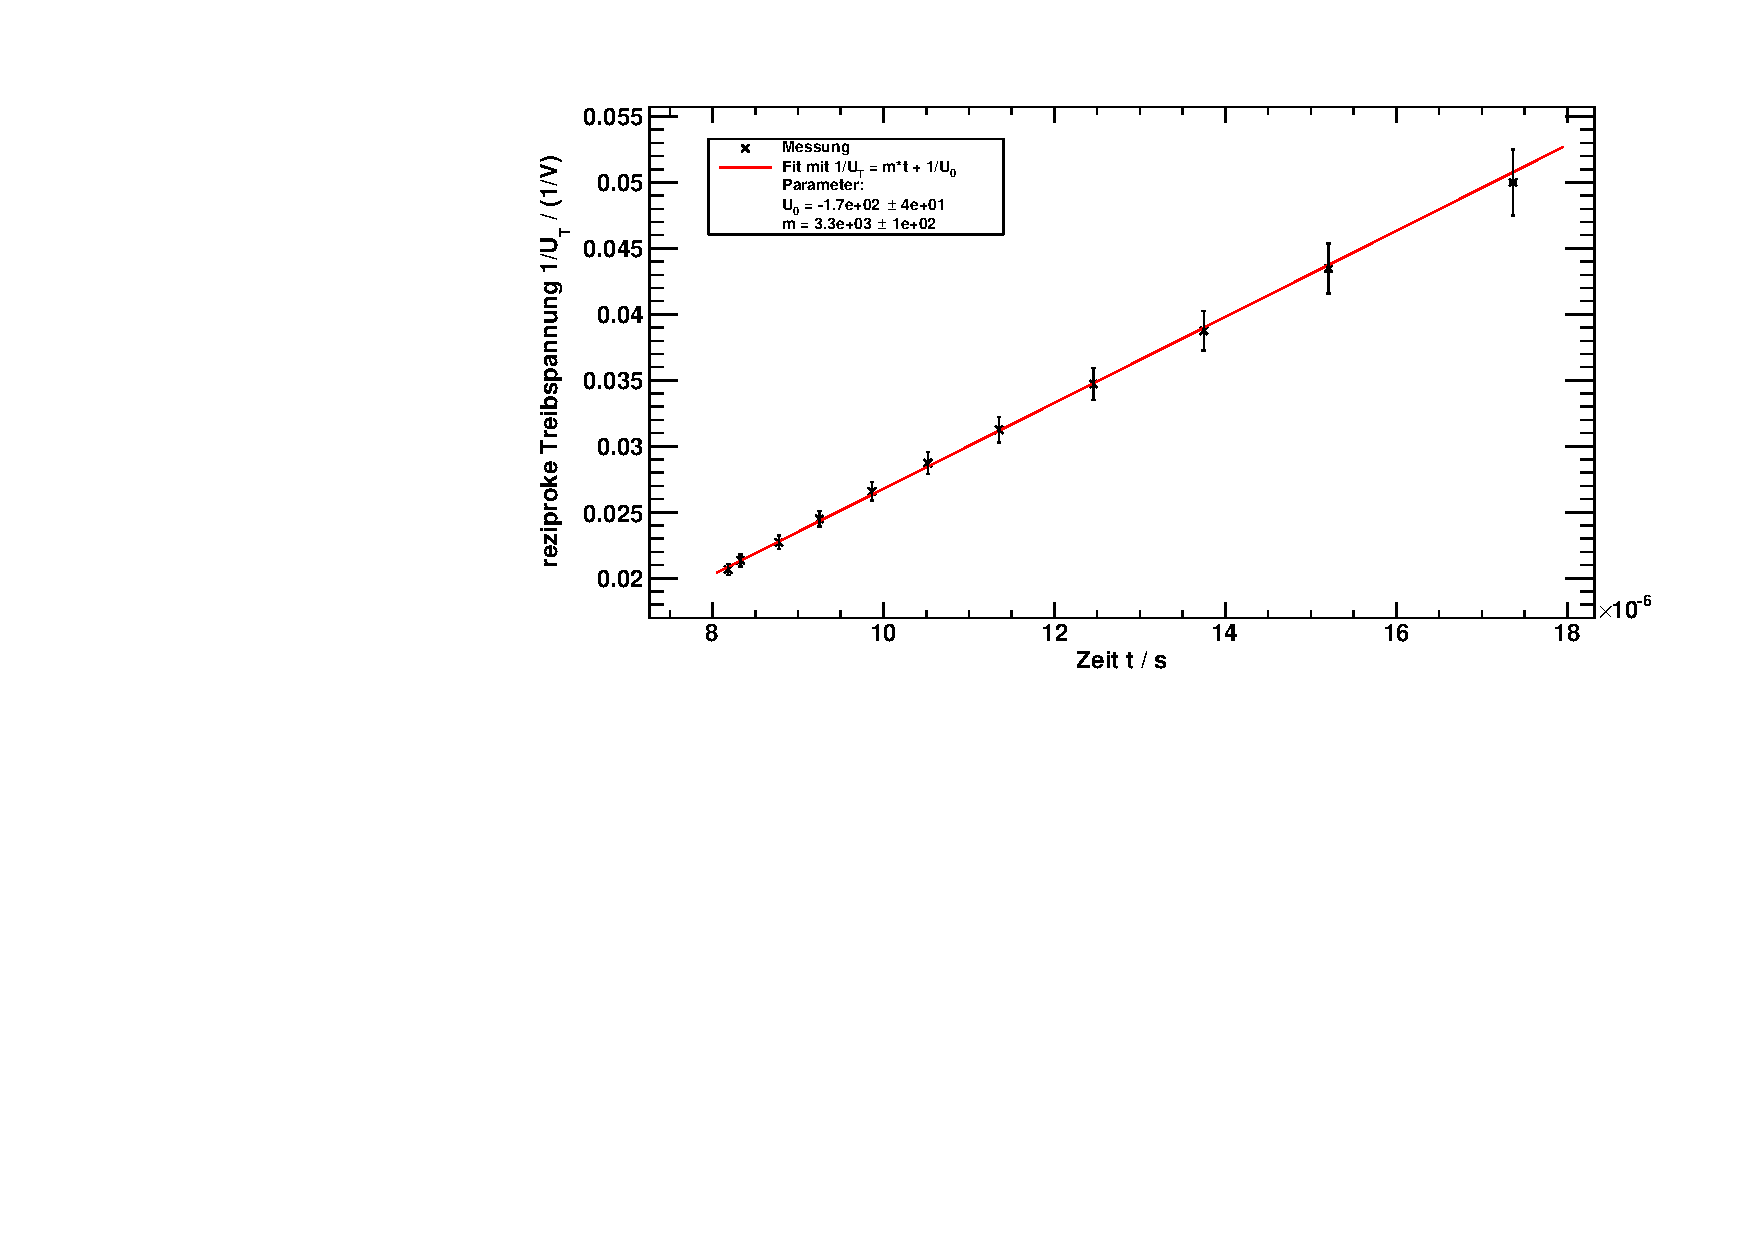
\includegraphics[width=\textwidth]{../img/part2/volt_fitXc.pdf}
  \caption{caption}
  \label{img:volt:fitxc}
\end{center}
\end{figure}

\paragraph{Bestimmung der Diffusionskonstanten $D_\text{n}$}
Platzhalter

\begin{figure}[H]
\begin{center}
  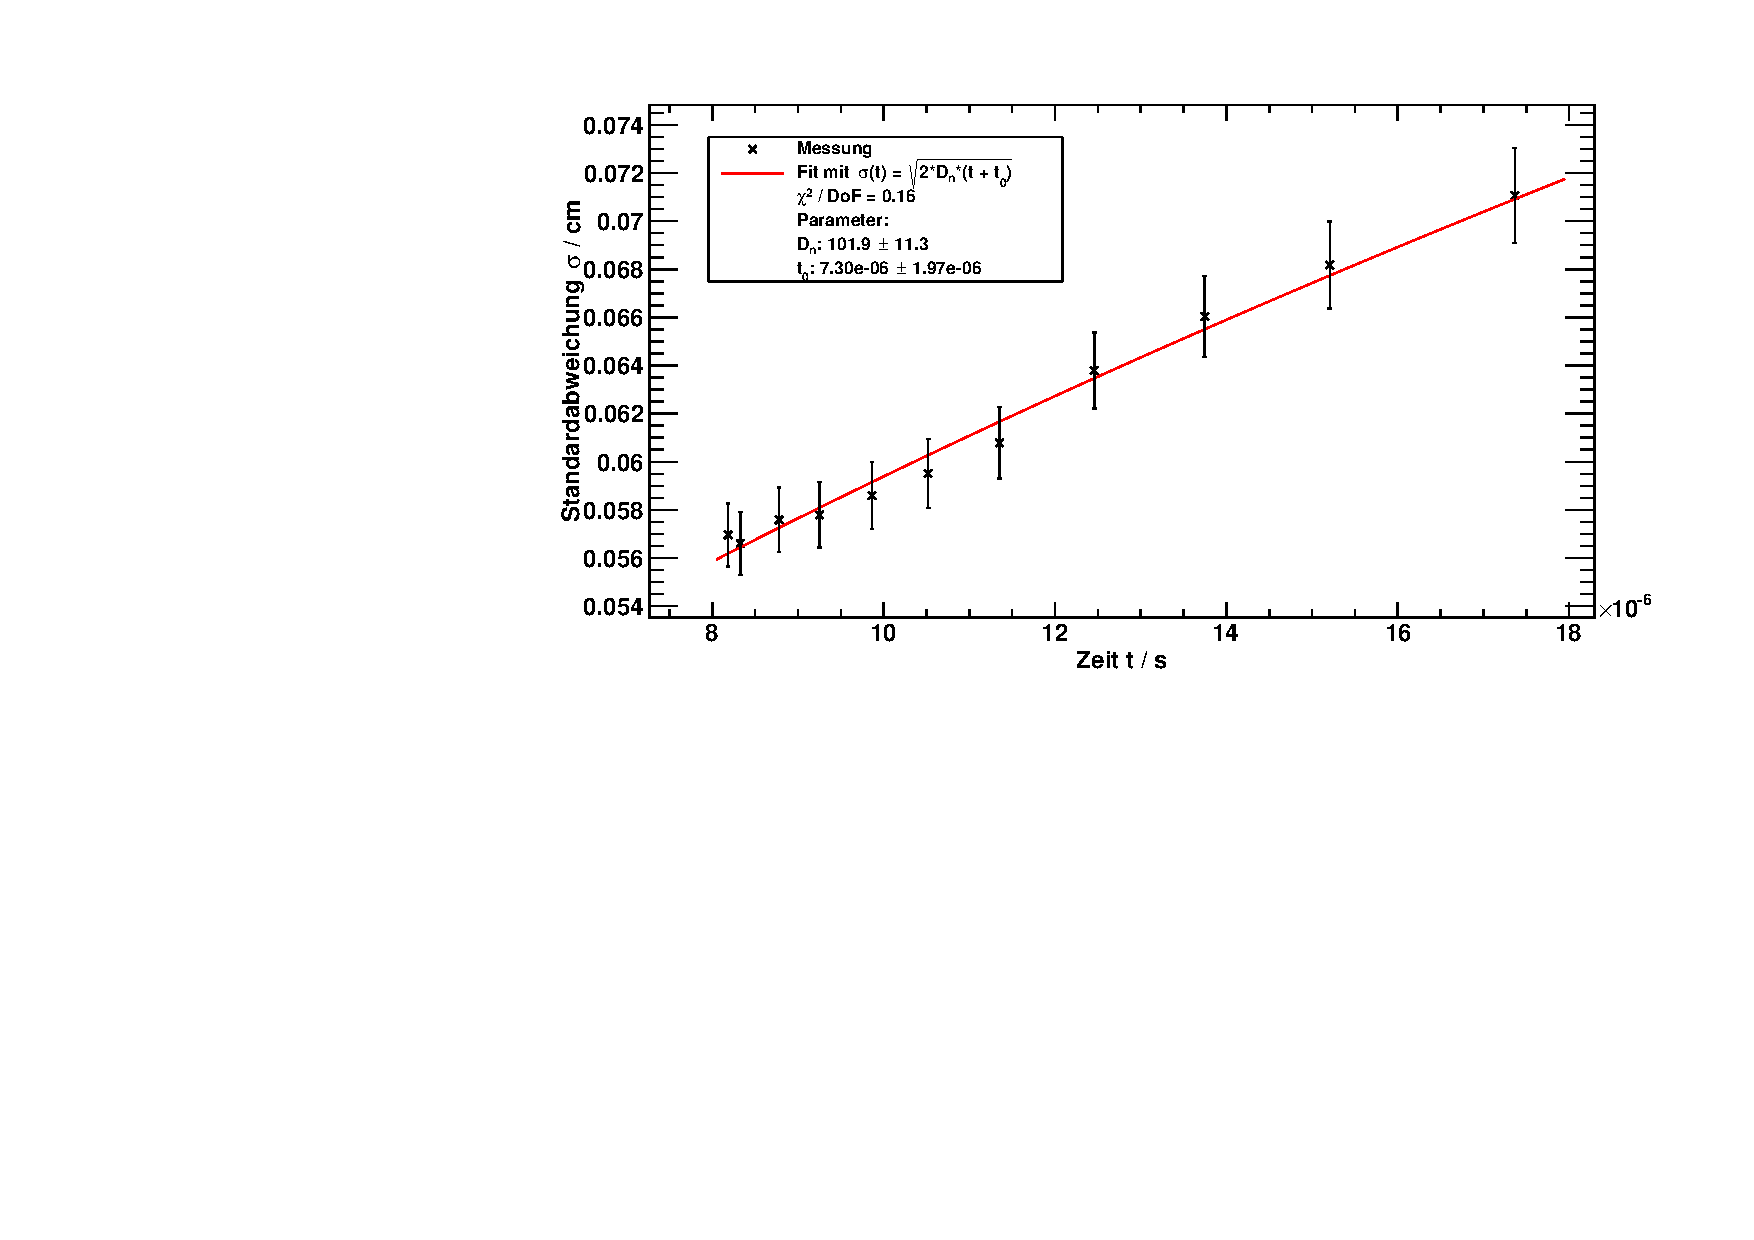
\includegraphics[width=\textwidth]{../img/part2/volt_fitSigma.pdf}
  \caption{caption}
  \label{img:volt:fitsigma}
\end{center}
\end{figure}

\paragraph{Bestimmung der mittleren Lebensdauer $\tau_\text{n}$}
Platzhalter

\begin{figure}[H]
\begin{center}
  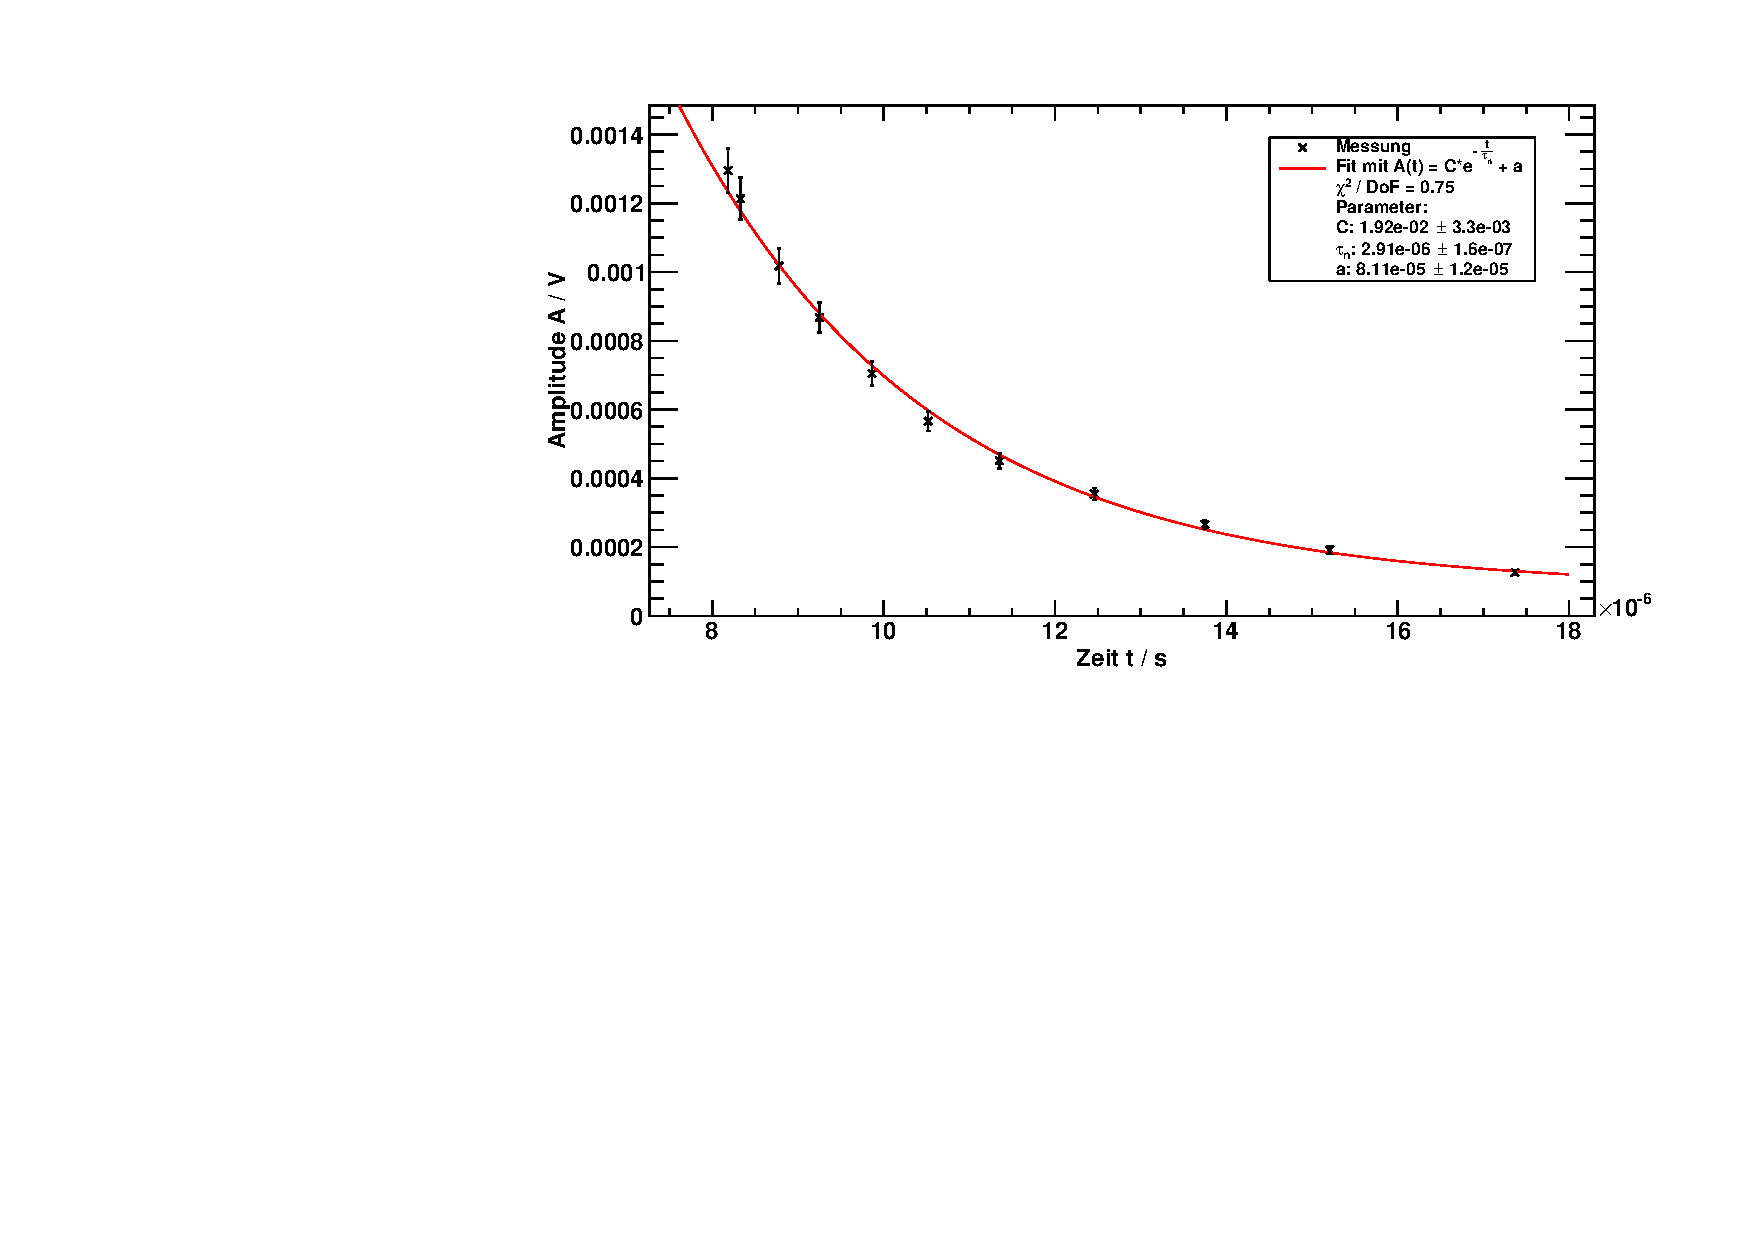
\includegraphics[width=\textwidth]{../img/part2/volt_fitA.pdf}
  \caption{caption}
  \label{img:volt:fita}
\end{center}
\end{figure}